\chapter{\gkchapter{La langue}{L’objet d’étude de la linguistique}}\label{sec:1.1}

\section{Parler une langue}\label{sec:1.1.0}

Pour comprendre ce qu’est une langue, il faut comprendre à quoi elle sert. Savoir \hi{utiliser une langue}, c’est être capable de parler dans cette langue et de comprendre ceux qui nous parlent. \hi{Parler une langue}, c’est être capable de verbaliser n’importe quelle idée, c’est-à-dire \hi{transformer un sens en un son} dont notre interlocuteur pourra lui-même extraire un sens (voir dans l’encadré qui suit le schéma proposé par Saussure). Si le sens de départ – celui pensé par le locuteur – et le sens d’arrivée – celui construit par le destinataire – sont suffisamment proches, alors, la \hi{communication} peut être considérée comme réussie.

La \textstyleTermes{langue} est donc avant tout un objet qui se trouve dans le \hi{cerveau} des locuteurs et que l’on peut modéliser par une \hi{correspondance entre des sens et des sons}. Plus exactement, nous modélisons la langue par une correspondance entre des représentations sémantiques et des textes. Dans la suite, nous utiliserons le terme \textstyleTermes{texte} pour désigner les productions langagières qu’elles soient orales, écrites ou gestuelles. Ce terme a l’avantage de ne pas présupposer quelle est la nature du médium utilisé pour communiquer. Il a également l’avantage sur le terme \textit{son} de renvoyer à une représentation du son et non au son lui-même. Un texte sonore est ainsi la représentation que nous avons du son dans notre cerveau lorsque nous produisons des sons afin de communiquer. L’étude même de la représentation du son — la \textstyleTermes{phonologie} — ne sera abordée que dans la mesure où elle interfère avec la syntaxe. Nous nous intéressons à la modélisation du mécanisme cognitif (situé dans le cerveau) et nous laissons de côté le mécanisme physique qui permet la production du son à partir du texte (cela concerne la phonétique articulatoire), ainsi que le mécanisme auditif qui permet le décodage du son.

Considérer que la langue est une correspondance, c’est faire abstraction des mécanismes propres à la production ou la compréhension d’un texte. Le locuteur utilise la correspondance du sens vers le texte, tandis que le destinataire effectue le chemin inverse. Nous supposons implicitement que les deux directions, sens vers texte et texte vers sens, utilisent le même ensemble de connaissances et un mécanisme commun, qui constituent la langue proprement dite.

\chevalier{La langue comme correspondance sens-texte}{
    On trouve déjà dans le \textit{Cours de linguistique générale} de Ferdinand de Saussure, publié en \citeyear{saussure1916cours}, la conception de la langue comme un objet qui fait se correspondre des sens et des «~sons~». Voici ce qu’il écrit :

    \begin{quote}
    «~Pour trouver dans l’ensemble du langage la sphère qui correspond à la langue, il faut se placer devant l’acte individuel qui permet de reconstituer le circuit de la parole. Cet acte suppose au moins deux individus ; c’est le minimum exigible pour que le circuit soit complet. Soient donc deux personnes A et B, qui s’entretiennent :\medskip\\
    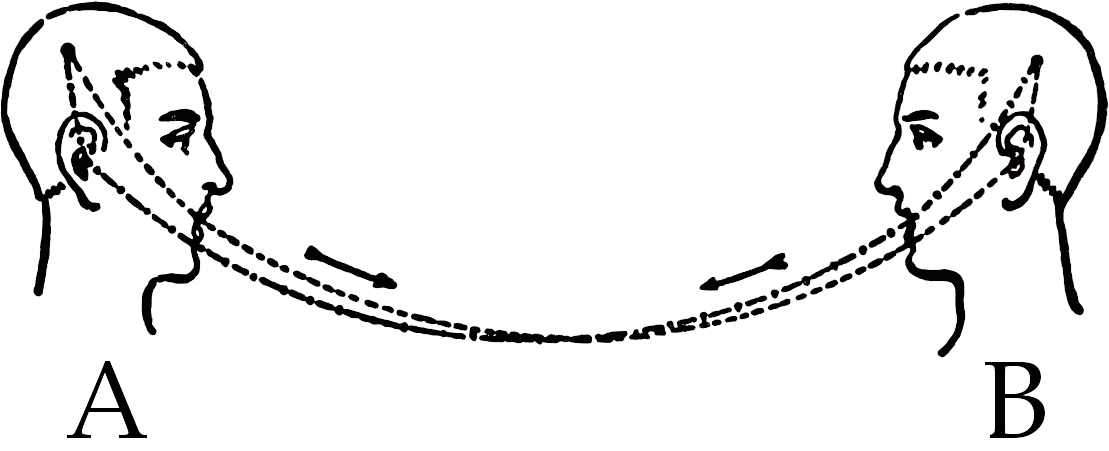
\includegraphics[width=\linewidth]{figures/vol1syntaxe2-img011.png}\medskip\\
    Le point de départ du circuit est dans le cerveau de l’une, par exemple A, où les faits de conscience, que nous appellerons concepts, se trouvent associés aux représentations des signes linguistiques ou images acoustiques servant à leur expression. Supposons qu’un concept donné déclenche dans le cerveau une image acoustique correspondante : c’est un phénomène entièrement \textit{psychique}, suivi à son tour d’un procès \textit{physiologique} : le cerveau transmet aux organes de la phonation une impulsion corrélative à l’image ; puis les ondes sonores se propagent de la bouche de A à l’oreille de B : procès purement \textit{physique}. Ensuite, le circuit se prolonge en B dans un ordre inverse : de l’oreille au cerveau, transmission physiologique de l’image acoustique ; \hi{dans le cerveau association psychique de cette image psychique avec le concept correspondant}. Si B parle à son tour ce nouvel acte suivra — de son cerveau à celui de A — exactement la même marche que le premier et passera par les mêmes phases successives.~» (\citealt{saussure1916cours} : 27--28) [c’est nous qui soulignons]
    \end{quote}

    Saussure insiste, quelques lignes plus loin, sur le fait que l’association entre sens et son qui a lieu dans le cerveau ne se fait pas avec le son lui-même, mais avec une représentation de ce son dans le cerveau, que Saussure nomme l’\hi{image acoustique~}:

    \begin{quote}
    «~[Il faut] distinguer les parties physiques (ondes sonores) des physiologiques (phonation et audition) et psychiques (images verbales et concepts). Il est en effet capital de remarquer que l’image verbale ne se confond pas avec le son lui-même et qu’elle est psychique au même titre que le concept qui lui est associé.~» (\citealt{saussure1916cours} : 28--29)
    \end{quote}

    Leonard \citet[27]{bloomfield1933language}, le père de la linguistique américaine, va dans le même sens :

    \begin{quote}
    «~On produit de nombreuses sortes de bruits vocaux dont on utilise la variété : sous certains types de stimuli, on produit certains sons vocaux et nos compagnons, entendant les mêmes sons, font la réponse appropriée. Pour le dire brièvement, dans la parole humaine, des sons différents ont des sens différents. \hi{Étudier} \hi{la coordination de certains sons avec certains sens,} \hi{c’est} \hi{étudier la langue.}~» [nous soulignons] (Voir les \textit{Citations originales} en fin de chapitre.)
    \end{quote}

    Le fait de considérer que l’objet d’étude de la linguistique est de modéliser la correspondance sens-son décrite par Saussure (et appelée par lui association concept-image acoustique) peut être imputé à Žolkovskij et Mel’čuk qui posent en \citeyear{zolkovski1967semanticeskom} à Moscou les bases de la Théorie Sens-Texte, dont le nom même est tout à fait explicite sur ce point. Dans son cours au Collège de France en \citeyear{melcuk1997vers} intitulé \textit{Vers une linguistique Sens-Texte}, Igor Mel’čuk pose qu’un modèle d’une langue est une correspondance multivoque entre un ensemble de sens et un ensemble de textes, où les textes désignent les images acoustiques des phrases de la langue. Le caractère multivoque est dû au fait qu’un même sens peut être exprimé par différents textes (qui sont alors des «~paraphrases~» les uns des autres) et qu’un texte peut avoir plusieurs sens (c’est-à-dire être sémantiquement ambigu).

    Cette conception de la langue comme une correspondance sens-son est maintenant partagée par la plupart des théories, y compris par la grammaire générative de Noam Chomsky, qui pose, depuis le \textit{programme minimaliste} élaboré dans les années 1990 (voir \cite{chomsky1995minimalist}), qu’un modèle linguistique doit relier sens et sons.
}
\section{Sons et textes}\label{sec:1.1.2}

Il n’est jamais inutile de rappeler que les langues sont avant tout orales (ou gestuelles comme les langues des signes) et que l’écrit n’est qu’une \textstyleTermes{transcription}, nécessairement imparfaite et partielle, des productions orales, même s’il tend à avoir son autonomie et à acquérir sa propre codification. D’après Leonard \citet{bloomfield1933language}, «~L’écrit n’est pas la langue, mais simplement une façon d’enregistrer la langue au moyen de marques visibles. Une langue est la même quel que soit le système d’écriture utilisé pour l’enregistrer, exactement comme une personne est la même quelle que soit la façon dont on prend son image.~» (Nous traduisons en français toutes les citations. Voir les citations originales en fin de chapitre.) La même idée est reprise par H. A. \citet{gleason1955introduction} : «~Une langue écrite est typiquement un reflet, indépendant sous quelques aspects seulement, des langues parlées. En tant qu’image de la parole réelle, elle est inévitablement imparfaite et incomplète. […] La linguistique doit commencer par une étude approfondie de la langue parlée avant d’étudier la langue écrite. C’est vrai pour des langues avec une longue tradition écrite, comme l’anglais, autant que pour les langues de tribus isolées qui n’ont jamais envisagé la possibilité d’une écriture.~» Cent ans avant (dans son ouvrage sur la langue kavi publié en \citeyear{humboldt1836uber}), le philosophe et linguiste Wilhelm von Humboldt écrivait que « la langue, comprise dans son essence réelle, est quelque chose de constant et à la fois, à tout moment, quelque chose de passager. Même sa conservation par l’écriture n’est jamais autre chose qu’un stockage ressemblant à une momie, qui nécessite qu’on cherche à s’imaginer à nouveau le discours vivant.~» Cette primauté de l’oralité est constitutive des sciences du langage et la distingue fondamentalement des lettres et de la philologie (l’étude des textes écrits). Les scientifiques n’en ont néanmoins réellement pris conscience qu’au début du vingtième siècle avec les possibilités nouvelles que donnait l’enregistrement des sons et l’intérêt croissant pour les langues sans tradition écrite et notamment les langues amérindiennes ; la linguistique s’était jusque-là, à l’exception des travaux des missionnaires qui avaient pour mission d’enseigner la Bible dans des langues inconnues, essentiellement développée par l’étude de langues mortes dont on ne conservait que des traces écrites que l’on souhaitait déchiffrer.

Certaines caractéristiques essentielles des langues sont dues au fait que ce sont des modes de communication oraux. La principale de ces caractéristiques est que la communication orale impose une production linéaire : la \textstyleTermes{chaîne parlée} est \hi{unidimensionnelle}. Les sons doivent être produits les uns à la suite des autres. L’écrit n’imposerait pas cela. La communication écrite fait d’ailleurs un grand usage de schémas bidimensionnels souvent complexes et la présentation globale d’un texte écrit (titres, paragraphes, encadrés, etc.) joue un rôle non négligeable. Néanmoins, l’écrit traditionnel, et parce qu’il est au départ une transcription de l’oral, a une organisation linéaire, les mots devant se lire à la suite les uns des autres. On notera qu’aujourd’hui, avec l’internet, les textes contiennent une multitude de liens vers d’autres textes et qu’une production textuelle faite de plusieurs pages web n’est plus totalement linéaire : il a une structure en réseau et on parle alors d’\textstyleTermes{hypertexte}. Cette organisation, qui permet différents parcours du texte, existe déjà en partie dans les écrits traditionnels par la présence de notes ou d’encadrés.

Les langues des signes n’ont pas de contraintes de linéarité, puisque les gestes peuvent se développer dans toutes les dimensions de l’espace et différentes parties du corps être utilisées simultanément (mains, position de la tête, regard, orientation du buste, etc.). Il y a néanmoins une contrainte temporelle dans la communication qui veut qu’il y ait une certaine séquentialité des signes.

Le caractère linéaire de la chaîne parlée est lui-même en partie contourné par l’utilisation de la \textstyleTermes{prosodie~}: les locuteurs ajoutent à la suite des sons distinctifs élémentaires qu’ils produisent — les \textstyleTermes{phonèmes} — de l’information en modulant leur mélodie et en jouant sur l’intensité du signal et la durée des phonèmes. Ceci permet non seulement de communiquer certaines émotions, mais aussi de structurer la chaîne parlée en faisant apparaître des regroupements ou des changements de plan. On retrouve à l’écrit une transcription de la prosodie par la \textstyleTermes{ponctuation} (point, virgule, :, ?, !).  On peut imaginer qu’un langage purement écrit aurait développé un tout autre système et on voit que la ponctuation n’est rien d’autre qu’un marquage partiel et imparfait de la prosodie. On notera que, avec le récent développement du dialogue par écrit, le système de ponctuation s’est enrichi des smileys, émojis et autres émoticônes (\HappySmiley{}, \SadSmiley{}, et plein d’autres).

Nous aurons plusieurs fois l’occasion dans cet ouvrage de montrer que les faits de langue se comprennent bien mieux lorsqu’on se place du côté de l’oral et que notre objet d’étude est d’abord la langue parlée, même si, par commodité, dans un ouvrage écrit, il est souvent plus facile de donner des exemples écrits.

\globe{Langue et variations}{%\label{sec:1.1.3}
     On observe de nombreuses variations entre locuteurs d’une même langue : accent, choix lexicaux, constructions grammaticales, etc. Ces variations sont dues à de multiples facteurs : le degré d’apprentissage de la langue, l’époque à laquelle vit le locuteur, le lieu où il vit, le contexte social dans lequel il s’exprime (la famille, le travail, la radio …), etc. Ainsi l’allemand est pris entre deux langues très proches, le néerlandais et le suisse allemand et on observe un continuum de variétés d’allemand lorsqu’on se rapproche de ces deux zones linguistiques. Pour le français, on observe également des différences de parler suivant les régions, entre le nord et le sud de la France (le système phonologique, notamment, est différent), mais aussi entre la France, la Belgique, la Suisse, le Québec ou les pays francophones d’Afrique. Et à chaque fois, on observe un continuum de parler entre divers extrêmes. Il en va de même pour l’évolution des langues : la limite entre le latin et les langues romanes d’aujourd’hui (italien, espagnol, catalan, français, roumain, corse, etc.) n’est pas une frontière tranchée : le latin a évolué de génération en génération jusqu’à perdre ses désinences casuelles (qu’on ne retrouve dans aucune des langues romanes), puis divers groupes de locuteurs du haut-latin se sont retrouvés isolés au Moyen-Age et ont développés les dialectes que sont nos langues d’aujourd’hui. Le français, ancienne langue d’oïl, a subi l’influence de locuteurs d’origine germanique et la syntaxe de l’ancien français est beaucoup plus proche de celle des langues germaniques d’aujourd’hui (allemand, néerlandais, scandinave) que du latin classique. La situation est identique partout. Si l’on appelle chinois aussi bien le chinois classique que le mandarin actuel, ces langues n’en sont pas moins éloignés que le latin et l’italien. Il existe d’ailleurs aujourd’hui en Chine au moins quatre langues différentes, qui bien que partageant la même écriture, sont plus différentes entre elles que ne le sont les langues romanes entre elles.

    D’une certaine façon, ces variations ne nous intéressent pas : nous décrivons un système unique, celui d’un locuteur donné à un moment donné ou au moins la langue d’un groupe de locuteurs qui communiquent usuellement entre eux. Ce qui nous intéresse avant tout, c’est la cohérence interne de ce système. Néanmoins, les variations possibles de ce système peuvent parfois nous intéresser : elles nous permettent en particulier de comprendre certaines «~bizarreries~» du système qu’on ne saurait expliquer sans prendre en compte le fait qu’il s’agit d’un système en évolution. Par exemple, la non-correspondance entre les unités de forme et les unités de sens (question que nous développerons en long et en large dans la partie 2 consacrée aux \textit{Unités de la langue}) ne peut s’expliquer sans prendre en compte comment de nouveaux termes sont créés par les locuteurs et comment d’autres disparaissent. Il faut d’ailleurs distinguer deux types de changements dans les langues : les changements lexicaux et les changements grammaticaux. Tout locuteur modifie constamment son vocabulaire, acquérant de nouvelles unités lexicales et cessant d’en utiliser certaines. Par contre, il est peu probable qu’une fois l’enfance passée et l’acquisition complète de la grammaire effectuée des changements se produisent dans le système grammatical. Il est plus raisonnable de penser que les changements grammaticaux ont lieu lors du passage de relais d’une génération à l’autre : pour une raison ou une autre, l’apprenant va faire une analyse différente des productions langagières de ses «~instructeurs~» et construire une grammaire différente de la leur. Le cas le plus radical est celui d’un groupe d’apprenants d’une autre langue maternelle qui va projeter sur la langue qu’il apprend des constructions de sa langue maternelle. Les langues romanes et tout particulièrement l’ancien français sont ainsi des formes du latin dont une partie de l’évolution est due à l’assimilation d’apprenants de langue germanique.
}
\section{Sens et intention communicative}\label{sec:1.1.4}

Notre définition de la langue n’est compréhensible que si on s’entend quelque peu sur ce qu’est le sens. Pour cela nous allons partir de la définition que donne Leonard Bloomfield dans \textit{Language}, son ouvrage fondateur de 1933.

Pour Bloomfield, il y a \textstyleTermes{acte de langage} lorsque Jill a faim, qu’elle voit une pomme dans un arbre et qu’au lieu de grimper dans l’arbre la cueillir, elle produit un son avec son larynx, sa langue et ses lèvres et que c’est Jack qui cueille la pomme et la lui apporte. Autrement dit, face à un stimulus S (Jill a faim et voit une pomme), il y a deux voies pour arriver à la réaction R :

\begin{itemize}
\item 
la voie directe S → R, où Jill grimpe dans l’arbre,
\item 
et la voie indirecte S → \begin{tikzpicture}[baseline=(r.base)] \node at (0,0) (r) {r}; \node[right=1em of r] (s) {s}; \draw[dashed,thick] (r) -- (s);\end{tikzpicture} → R, où une réaction linguistique r se substitue à la réaction mécanique de Jill et où le stimulus s qu’elle provoque donne la réaction R chez Jack.
\end{itemize}

Reprenons la citation de Bloomfield, donnée dans l’\encadref{fig:1.1.1} sur \textit{La langue comme correspondance sens-texte}, sous ce nouvel éclairage :

\begin{quote}
    «~On produit de nombreuses sortes de bruit vocaux dont on utilise la variété : sous certains types de stimuli, on produit certains sons vocaux et nos compagnons, entendant les mêmes sons, font la réponse appropriée. Pour le dire brièvement, dans la parole humaine, des sons différents ont des sens différents. Étudier la coordination de certains sons avec certains sens, c’est étudier la langue.~» (\citealt{bloomfield1933language} : 27)
\end{quote}

\noindent Jusque-là, nous sommes parfaitement d’accord. Reste à définir le sens :

\begin{quote}
    «~En produisant une forme linguistique, un locuteur incite son interlocuteur à répondre à une situation ; cette situation et la réponse qu’elle déclenche sont le \textit{sens linguistique} de la forme. Nous supposons que chaque forme linguistique a un sens constant et défini, différent du sens de n’importe quelle autre forme linguistique de la même langue.~» (\citealt{bloomfield1933language} : 165)
\end{quote}

\noindent Là, nous ne sommes plus en accord. Nous pensons qu’il faut absolument séparer la situation du sens linguistique. Dans la même situation, Jill peut produire des énoncés de sens différents comme «~\textit{Pourrais-tu} \textit{me cueillir cette pomme} ?~» ou «~\textit{Apporte-moi cette pomme !~}» ou des énoncés moins coercitifs comme «~\textit{J’ai faim.}~» ou «~ \textit{Regarde cette belle pomme !~}», qui peuvent néanmoins amener la même réaction de Jack. Inversement, dans une tout autre situation, par exemple face à une nature morte dans un musée, Marie peut dire à Pierre «~\textit{Regarde cette belle pomme} !~» et cet énoncé a, pour notre définition du sens, le même sens que l’énoncé «~\textit{Regarde cette belle pomme} !~» de Jill, qui procédait pourtant d’intentions complètement différentes.

Autrement dit, nous distinguons clairement trois objets :

\begin{itemize}
\item le \textstyleTermes{contexte d’énonciation}, c’est-à-dire les caractéristiques extérieures de la situation où est produit l’énoncé : qui parle à qui ? où et quand ? dans quelles circonstances ? etc.
\item les \textstyleTermes{intentions communicatives} du locuteur, c’est-à-dire les buts que se fixe le locuteur, les informations qu’il souhaite communiquer sur tel ou tel objet dans le contexte, etc.
\item le \textstyleTermes{sens linguistique} de l’énoncé, c’est-à-dire, indépendamment du contexte et des intentions du locuteur, le contenu de son message, les éléments de sens qu’il a choisi pour communiquer l’information, désigner tel objet, etc. Le sens linguistique, tel que nous l’envisageons, est très proche du texte, puisqu’il contient déjà les sens des différentes unités du texte.
\end{itemize}

La phase d’élaboration du contenu d’un message, c’est-à-dire le passage d’intentions communicatives dans un contexte donné à un sens linguistique s’appelle la \textstyleTermes{planification} du message. On considère généralement que l’étude de la planification ne relève pas de la linguistique et que cette étape reste relativement indépendante du langage, dans la mesure où toutes les langues permettent d’exprimer à peu près tous les sens (comme le montre l’absence d’obstacles majeurs à la traduction d’une langue à l’autre, sauf lorsqu’il s’agit de concept absent d’une culture à l’autre). Laurence \citet{danlos1987generation}, l’une des pionnières de la génération automatique de textes, propose d’appeler la planification le \textit{Quoi dire}, qu’elle oppose au \textit{Comment le dire}, qui constitue la langue proprement dite.

Nous savons bien sûr que la planification est en partie guidée par le stock lexical que chaque langue propose et nous allons voir un peu plus loin (\sectref{sec:1.1.9}) que la planification joue quand même un rôle dans l’organisation des énoncés et la syntaxe, même si dans cet ouvrage nous étudierons essentiellement le passage du sens au texte. L’étude même des sens linguistiques — la \textstyleTermes{sémantique} — ne sera abordée que dans la mesure où elle interfère avec la syntaxe.

\loupe{Mots et pensée}{%\label{sec:1.1.5}
    La question se pose de savoir si on peut penser sans mots, c’est-à-dire si on peut manipuler des concepts sans les verbaliser, même dans sa tête. Nous pensons que oui. Le bricoleur qui répare son moteur pense à toutes les pièces du moteur qu’il manipule sans avoir nécessairement une idée de comment les appeler et il effectue un grand nombre d’actions bien réfléchies qu’il aurait bien du mal à expliquer en mots. Plus on va vers une pensée abstraite, plus on pourrait penser que les sens doivent se confondre avec les mots. Pourtant, le mathématicien qui fait une démonstration n’a pas toujours les mots pour exprimer les concepts qu’il manipule et une part de son activité est justement d’isoler ces concepts et de leur donner des noms : ensemble, fonction, continuité, etc. Ici il est clair que le concept précède dans la pensée le terme qui lui correspond. Nous faisons l’hypothèse qu’il existe une forme abstraite de pensée sans mots et que la langue est l’ensemble des connaissances qui nous permet d’exprimer cette pensée. Cette hypothèse reste aujourd’hui plus ou moins invérifiable et est controversée. Pour une discussion très lisible de ces idées, voir l’ouvrage de Steven \citet{pinker1997how} sur \textit{Comment fonctionne l’esprit}.
}
\globe{Sens lexicaux et traduction}{%\label{sec:1.1.6}
    Les sens exprimables par des mots simples varient d’une langue à l’autre, ce qui élimine tout espoir de traduction exacte. Par exemple, l’anglais possède une unité lexicale \textsc{melon} qui dénote aussi bien le melon que la pastèque et le français ne possède pas d’équivalent. Le verbe \textsc{esperar} de l’espagnol couvre à la fois les sens ‘espérer’ et ‘attendre’ du français et il existe un continuum entre les deux sens : ‘esperar’ ne sera donc pas ambigu mais «~sous-spécifié~» en ce qui concerne le degré de joie et de certitude qu’a la personne qui «~\textit{espera~}». À l’inverse, le verbe \textsc{aimer} couvre ce que l’anglais exprime avec \textsc{love} et \textsc{like}, car encore une fois, les locuteurs du français considère un continuum entre ces sens. Il existe aussi des sens lexicaux propres à une langue : par exemple, le nom allemand \textsc{schadenfreunde} désigne la joie que procure le dépit mérité des autres et n’a pas d’équivalent en français, bien que le concept puisse être universellement compréhensible. De la même façon, un verbe français comme \textsc{s’accouder} n’aura pas de meilleur équivalent dans beaucoup d’autres langues (par exemple en anglais ou en allemand) qu’une traduction littérale de ‘s’appuyer sur les coudes’.
}
\section{Langue, linguistique et modélisation}\label{sec:1.1.7}

Nous allons définir un certain nombre de termes dont nous aurons besoin et que nous avons déjà commencé à utiliser.

\Definition{\textstyleTermes{locuteur}, \textstyleTermes{sujet parlant}, \textstyleTermes{destinataires}, \textstyleTermes{interlocuteurs}}{Un \textstyleTermes{locuteur} ou \textstyleTermes{sujet parlant} est quelqu’un qui parle, c’est-à-dire quelqu’un qui cherche à communiquer avec d’autres gens en produisant des paroles ou un texte écrit. Il s’adresse à des \textstyleTermes{destinataires} ou \textstyleTermes{interlocuteurs}.}

\Definition{\textstyleTermes{langue}}
{Une \textstyleTermes{langue} est un système de signes conventionnels partagés par un certain nombre de personnes et qui leur permet de communiquer entre elles. Ces signes s’assemblent pour former des mots, des phrases et des discours. Une langue est à la fois un \hi{objet individuel} — c’est l’ensemble des connaissances stockées dans notre cerveau qui nous permettent de parler (dans cette langue) — et un \hi{objet collectif} et \hi{social}, puisque ces connaissances sont partagées par un certain nombre de personnes, qui sont les locuteurs de cette langue.}

\Definition{\textstyleTermes{faculté langagière}, \textstyleTermes{la langue}}
{La \textstyleTermes{faculté langagière} est l’aptitude que nous avons à apprendre et utiliser les langues. Le cerveau est l’organe de la faculté langagière (avec le système phonatoire que le cerveau commande pour produire des sons). Lorsqu’on parle de \textstyleTermes{la langue}, et non plus d’une langue particulière, on fait généralement référence à la faculté langagière et ce qu’elle va imposer comme traits communs à l’ensemble des langues possibles.}

\Definition{\textstyleTermes{linguistique}}
{La \textstyleTermes{linguistique} est la science qui étudie les langues du monde. Comme beaucoup de scientifiques, nous considérons que la linguistique inclut l’étude de la faculté langagière, c’est-à-dire l’étude de la production langagière et de l’apprentissage d’une langue par l’enfant. La linguistique est alors quasiment une branche de la psychologie.}

La linguistique produit des \textstyleTermes{modèles des} \textstyleTermes{langues} et de la faculté langagière. Ces modèles doivent être capables de simuler un \textstyleTermes{acte de langage}, c’est-à-dire la façon dont un locuteur produit un texte à partir d’un sens qu’il veut exprimer et la façon dont son interlocuteur reconstruit un sens à partir de ce texte.

Tout modèle se situe dans un \textstyleTermes{cadre théorique}. Décider que la langue est une correspondance est un choix théorique. Décider ce qui est mis en correspondance par la langue, c’est-à-dire ce que sont la représentation sémantique et le texte relève aussi de choix théoriques. C’est le cadre théorique qui caractérise notamment l’objet d’étude. Pour reprendre une formule de \citet{saussure1916cours} devenue fameuse, «~Bien loin que l’objet précède le point de vue, on dirait que c’est le point de vue qui crée l’objet.~».

\loupe{Langue et parole, compétence et performance}{%\label{sec:1.1.8}
    Saussure oppose deux notions fondamentales qu’il nomme \textstyleTermes{langue} et \textstyleTermes{parole~}:

    \begin{quote}
    «~Entre tous les individus ainsi reliés par le langage, il s’établira une sorte de moyenne : tous reproduiront, — non exactement, mais approximativement — les mêmes signes unis aux mêmes concepts. […]

    La {langue} n’est pas une fonction du sujet parlant, elle est le produit que l’individu enregistre passivement. […] Elle est la partie sociale du langage, extérieure à l’individu, qui à lui seul ne peut ni la créer ni la modifier ; elle n’existe qu’en vertu d’une sorte de contrat passé entre les membres de la communauté. […]

    La {parole} est au contraire un acte individuel de volonté et d’intelligence, dans lequel il convient de distinguer :

    1° les combinaisons par lesquelles le sujet parlant utilise le code de la langue en vue d’exprimer sa pensée personnelle ;

    2° le mécanisme psycho-physique qui lui permet d’extérioriser ces combinaisons.~»\\
    (\citealt{saussure1916cours} : 29-31)
    \end{quote}

    La parole, au sens de Saussure, couvre deux notions qu’il convient de séparer. Nous préférons parler de \textstyleTermes{productions langagières} pour la première notion, c’est-à-dire les énoncés réellement produits par des sujets parlants, tandis qu’on préférera appeler la deuxième notion la \textstyleTermes{faculté langagière}. Alors que la parole est un objet individuel, la \textstyleTermes{langue} est un objet social par excellence, mais c’est aussi la trace qu’a imprimée cet objet dans le cerveau de chacun de nous, objet collectif, donc, qui n’existe que par la somme de ses traces individuelles.

    L’opposition entre compétence et performance proposée par \citet{chomsky1965aspects} nous renvoie à l’opposition entre langue et parole, mais il convient de les distinguer : la compétence ne se confond pas avec la langue, ni la performance avec la parole. La \textstyleTermes{compétence} désigne notre compétence passive à savoir utiliser la langue, mais aussi à l’acquérir. Elle se divise en une compétence innée, qui peut se confondre avec la faculté langagière, et une compétence acquise, qui peut se confondre avec la langue en tant que trace individuelle d’une langue dans notre cerveau.

    La \textstyleTermes{performance} est l’usage proprement dit de la langue. La \textstyleTermes{parole} est le produit de la compétence et de la performance : nous avons la compétence de produire des énoncés supposément parfaits, mais divers facteurs (notre état émotionnel, des éléments qui vont nous distraire, la recherche d’un message approprié, etc.) vont faire que notre énoncé ne sera pas aussi parfait qu’il aurait pu l’être. Ceux qui veulent décrire la langue, comme nous, vont essayer de séparer ce qui relève d’un \textstyleTermes{manque de compétence} de ce qui relève d’une \textstyleTermes{erreur de performance}. La chose est loin d’être évidente, notamment lorsqu’on touche aux \textstyleTermes{limitations mémorielles}. Par exemple, Chomsky a beaucoup insisté sur le caractère \textstyleTermes{récursif} de la langue : une proposition peut contenir une proposition subordonnée (\textit{La personne} [\textit{que le chien a mordu}] \textit{est à l’hôpital}) et un tel enchâssement peut être itéré (\textit{La personne} [\textit{que le chien} [\textit{auquel le garçon a donné un os}] \textit{a mordu}] \textit{est à l’hôpital}). Mais cette dernière phrase est difficilement compréhensible et une insertion de plus dépasse nos capacités d’analyse en situation de communication ordinaire (\textit{La personne que le chien auquel le garçon qui habite au coin de la rue a donné un os a mordu est à l’hôpital}). Défaut de compétence ou de performance ? (Voir Exercice 3.)
}
\section{La planification}\label{sec:1.1.9}

Nous voudrions montrer ici que la planification (voir définition dans la \sectref{sec:1.1.4} sur \textit{Sens et intention communicative}) peut avoir des incidences non négligeables sur la nature du texte produit et que dans l’absolu il faut l’inclure dans notre objet d’étude. En particulier, on ne peut pas en général considérer que le locuteur construit le contenu de son message avant de le transformer en un énoncé, c’est-à-dire qu’il planifie complètement avant de produire un énoncé. Les choses ne se passent généralement pas comme ça et le locuteur élabore le contenu de son message au fur et à mesure de l’énonciation. Les productions orales présentent en particulier de nombreux indices de la planification en cours. (C’est moins net à l’écrit, puisque le scripteur à la possibilité de revenir en arrière pour corriger sa production.) Comme le dit Claire \citet[17]{blanche-benveniste1990francais}, «~Lorsque nous produisons des discours non préparés, nous les composons au fur et à mesure de leur production, en laissant des traces de cette production. […] L’étude de ces traces est en elle-même un sujet d’observations ; on y voit la production de langage en train de se faire. […] Une observation attentive permet de voir comment nous procédons, quelles unités nous utilisons pour faire avancer nos discours, quelles tenues en mémoire nous avons, à la fois pour les morceaux déjà énoncés et pour ceux que nous projetons d’énoncer. On peut ainsi observer comment se fait la mise au point des syntagmes, la recherche des «~bonnes dénominations~», et le travail constant d’évaluation que nous faisons sur nos propres discours.~»

Nous allons montrer trois phénomènes qui illustrent l’influence de la planification sur la structure de l’énoncé. Les exemples qui suivent sont des retranscriptions fidèles de productions orales attestées ; dans ces transcriptions figurent absolument tous les mots prononcés par le locuteur, y compris les bribes et répétitions dues aux hésitations du locuteur.

Les premiers indices de la planification en cours sont les nombreuses amorces que le locuteur fait et auxquelles il renonce momentanément ou définitivement. Dans l’exemple suivant, la locutrice semble ne pas trouver tout de suite la bonne formulation ; elle hésite et répété \textit{les} pour se donner du temps, amorce la production de \textit{les capitales}, mais s’y prend quand même à deux fois pour finalement proposer une reformulation par \textit{les grandes villes} :

\ea\itshape et je voulais pas aller à Addis Abeba puisque \textbf{les les les les c-} \textbf{les capitales les grandes villes} ne me disaient rien du tout\z

À chaque fois, on obtient une \textstyleTermes{bribe}, c’est-à-dire un segment inachevé qui est ensuite corrigé par le locuteur. La disposition suivante du texte, dite \textstyleTermes{analyse en grille}, permet de mettre en évidence l’\textstyleTermes{entassement} (voir le \chapref{sec:5.5}) dans la même position syntaxique de la bribe et du segment qui vient la remplacer :

\ea \begin{tabularx}{\linewidth}[t]{@{}l|>{\hangindent=1em}Q@{}}
et je voulais pas aller à AA puisque  & \textbf{les}\\
                                      & les\\
                                      & les\\
                                      & les c-\\
                                      & les capitales\\
                                      & \textbf{les grandes villes} ne me disaient rien du tout
    \end{tabularx}
\z

Plus étonnant est le phénomène de la \textstyleTermes{greffe} bien étudié par José Deulofeu (voir la partie 6). L’exemple suivant en fourni deux :

\ea
on avait critiqué le le journal de je crois que c’était le Provençal on l’avait critiqué par rapport à ou le Méridional par rapport à la mort de comment il s’appelle … pas Coluche l’autre

%%[Warning: Draw object ignored]
\z

À deux reprises, ici, le locuteur ne trouve pas le nom qu’il cherche et il vient greffer un énoncé qui pourrait fonctionner comme un énoncé autonome et qui est ici inséré dans l’énoncé principal dont il assure la complétion. Nous reprenons le texte précédent en le disposant selon les principes de l’analyse en grille et en indiquant les greffes en gras.

\ea \begin{tabular}[t]{@{}|l|l|l@{}}
on avait critiqué & \multicolumn{2}{l}{le}\\
                  & \multicolumn{2}{l}{le journal de}\\
                  & je crois que c’était  &  le Provençal\\
\multicolumn{1}{@{}|l}{} & \multicolumn{1}{l|}{} & \multicolumn{1}{l@{}}{}\\
on l’avait critiqué &  par rapport à & \\
\multicolumn{1}{@{}l|}{} &                & ou le Méridional\\
\multicolumn{1}{@{}l|}{} & \multicolumn{1}{l}{} & \multicolumn{1}{l@{}}{}\\
\multicolumn{1}{@{}l|}{} & par rapport à la mort de  &  \textbf{comment il s’appelle}\\
\multicolumn{2}{@{}c|}{} & pas Coluche\\
\multicolumn{2}{@{}c|}{} & l’autre             
\end{tabular}\todo[inline]{please check \& confirm}
\z

On notera que la première greffe s’entrelace avec l’énoncé principal, ce qui semble montrer que le locuteur poursuit en parallèle la planification de son énoncé principal et de la greffe. On voit à nouveau ici un fonctionnement par entassement de segments similaires ou identiques (\textit{on avait critiqué le journal - on l’avait critiqué, par rapport à - par rapport à}).

Un dernier phénomène illustre bien le fait que la planification a lieu en même temps que l’énonciation : les parenthèses. On appelle \textstyleTermes{parenthèse} tout énoncé qui vient s’insérer dans l’énoncé principal et qui est marqué par un changement de registre (une modification de l’intonation) qui le détache nettement de l’énoncé principal. Dans le texte suivant, nous avons indiqué les parenthèses entre parenthèses et nous avons directement disposé le texte en grille :

\ea donc pour essayer un petit peu de sortir cette personne de la misère (car c’est vraiment un petit peu semblable aux Misérables de Victor-Hugo) nous essayons tant bien que mal de lui faire comprendre que \textbf{sa cabane}\\
\begin{tabular}[t]{@{}|p{1cm}ll@{}}
    & \multicolumn{2}{|l}{dans quelques années (entre parenthèses, elle a 79 ans)}\\
    & \multicolumn{1}{|l}{quand elle aura} & \multicolumn{1}{|l}{des difficultés (ce qu’on espère pas)}\\
    & \multicolumn{1}{|l}{} & \multicolumn{1}{|>{\hangindent=1em}p{.55\textwidth}}{des difficultés à se déplacer ou à évoluer (c’est-à-dire qu’il y a énormément d’escaliers à monter pour arriver à sa cabane)}\\
    & \multicolumn{1}{|l}{donc le jour} & \multicolumn{1}{|l}{où elle ne pourra plus se déplacer}\\
    & \multicolumn{1}{|l}{} & \multicolumn{1}{|>{\hangindent=1em}p{.55\textwidth}}{ou qu’elle sera malade un petit peu plus sévèrement,}\\
    \multicolumn{3}{|>{\hangindent=1em}p{.85\textwidth}}{on essaye de lui faire comprendre qu’elle ne pourra plus vivre dans cette cabane}
\end{tabular}\todo[inline]{Kindly review \& comment}
\z

On peut résumer le contenu de ce texte ainsi : comme cette personne a 79 ans et qu’il y a énormément d’escaliers pour arriver à sa misérable cabane, il faut lui faire comprendre qu’elle ne pourra plus y vivre dans quelques années. On voit que deux informations essentielles (‘elle a 79 ans’ et ‘il y a énormément d’escaliers’) ont été ajoutées à la volée, ce qui a finalement obligé le locuteur à abandonner sa première proposition (\textbf{\textit{sa cabane}}, en gras dans le texte, est le sujet d’un verbe originalement planifié qui ne vient jamais) et à reprendre par une proposition équivalente (\textit{nous essayons tant bien que mal de lui faire comprendre que sa cabane} → \textit{on essaye de lui faire comprendre qu’elle ne pourra plus vivre dans cette cabane}). Il est probable qu’à la première lecture (qui aurait normalement dû être une écoute) de ce texte, vous ne vous êtes pas rendu compte que la première proposition avait été laissée inachevée : ceci montre le caractère très naturel de telles constructions et le fait que le destinataire est habitué à «~corriger~» les «~erreurs~» dues à la planification.

Les linguistes considèrent généralement que la planification est hors de leur objet d’étude et que la langue constitue uniquement le passage du contenu du message, c’est-à-dire le sens, à un énoncé. Les exemples précédents montrent que la planification, ou plutôt les problèmes de planification, laisse de nombreuses traces en surface et qu’il est donc difficile d’en faire abstraction, surtout si on étudie les productions orales. À l’écrit, par contre, les défauts de planification sont gommés par les passages successifs du rédacteur et la possibilité d’interrompre la rédaction pendant la planification. Ceci est encore une raison de préférer l’étude de l’oral à celle de l’écrit, car on trouve à l’oral davantage d’indices de la façon dont les locuteurs «~travaillent~», alors les corrections successives sont invisibles à l’écrit.

\section{Corpus et introspection}\label{sec:1.1.10}

Il existe deux moyens d’obtenir des faits de langue pour le linguiste. Le premier est de collecter des textes déjà produits. Un ensemble de textes est appelé un \textstyleTermes{corpus}. Le plus grand corpus disponible est le web et les moteurs de recherche constituent un assez bon moyen de récolter les données que l’on cherche, même s’il faut savoir trier ces données selon le type de page~(site d’information, blog, forum, chat, etc.) et le type d’auteur (locuteur natif, génération automatique, traduction automatique, etc.). Il existe des corpus plus spécialisés, comme les bibliothèques numériques d’ouvrages classiques, les archives des grands journaux, les encyclopédies en ligne ou les revues scientifiques. Les linguistes constituent des corpus pour leur besoin, notamment des corpus de productions orales dont les textes sont minutieusement retranscrits à l’écrit (nous en avons donné des exemples dans la section précédente). Certains de ces corpus concernent des populations particulières : enfants en phase d’acquisition, apprenants d’une seconde langue, aphasiques, etc. Tous ces paramètres constituent le \textstyleTermes{genre} de la production textuelle. Un bon corpus doit comporter ce type d’informations, qu’on appelle les \textstyleTermes{métadonnées}, c’est-à-dire les données qui concernent le corpus et se trouvent à côté des données proprement dites. En plus des métadonnées, certains corpus sont agrémentés d’annotations diverses permettant une meilleure étude des structures des énoncés. On trouve également des corpus alignés de différentes langues (qu’on appelle corpus multilingues ou bitextes) très utiles pour développer des modèles pour la traduction.

Le deuxième moyen d’étude est \textstyleTermes{l’introspection}. Il s’agit de construire artificielle\-ment des énoncés et d’en faire juger l’\textstyleTermes{acceptabilité} par des locuteurs natifs. Ce moyen permet de tester toutes les variantes imaginables d’un phénomène et surtout de vérifier les limites d’un phénomène en produisant des énoncés jugés inacceptables. Une autre raison qui peut justifier le recours à l’introspection est que, sur corpus, on rencontre beaucoup d’erreurs de performance, qui font que certains énoncés seraient jugés inacceptables même par ceux qui les ont produits. Il est donc nécessaire de garder un esprit critique et de savoir filtrer les résultats.

Un énoncé produit dans des conditions normales de production est dit \textstyleTermes{attesté}, par opposition à un énoncé \textstyleTermes{construit} par le linguiste. Même si nous ne rejetons pas l’introspection et l’appel au jugement des locuteurs, nous considérons que l’étude des corpus restent le meilleur moyen d’accéder aux données et d’éviter de passer à côté de phénomènes importants.

\section{Acceptabilité}\label{sec:1.1.11}
\subsection{Degrés d'acceptabilite}
Parmi toutes les phrases bizarres qu’un linguiste rencontre ou construit, il est souvent difficile de classer les phrases en bonnes et mauvaises. On constate plutôt une gradation de «~qualité~» qu’un jugement binaire en bon et mauvais.

Considérons les énoncés construits suivants :

\ea
\ea \itshape C’est un film que je sais que tu n’hésiteras pas une seconde à regarder.
\ex \itshape C’est un film que je me demande quand tu regarderas.
\ex \itshape C’est un film que je ne sais pas si tu accepteras que je regarde.
\ex \itshape C’est un film que je me demande jusqu’où tu es prêt à regarder.
\ex \itshape C’est un film que je dormais quand tu regardais.
\z
\z

On ressent facilement que la phrase (A) est meilleure que la phrase (B), qui elle-même est meilleure que (C). On constate que la phrase (E) est clairement inacceptable, tandis qu’on peut se demander si (D) l’est ou pas. Il est d’usage de noter l’\textstyleTermes{acceptabilité} des énoncés par des symboles allant de l’absence de symbole signifiant l’acceptabilité au symbole~* signifiant l’inacceptabilité, en passant par les symboles ? (léger doute), ?? (doute sérieux) et ?* (inacceptabilité probable). Pour nos exemples, nous aurions donc :

\ea
\judgewidth{\textsuperscript{?}*}
\ea[]{\itshape C’est un film que je sais que tu n’hésiteras pas une seconde à regarder.}
\ex[\textsuperscript{?}]{\itshape C’est un film que je me demande quand tu regarderas.}
\ex[\textsuperscript{??}]{\itshape C’est un film que je ne sais pas si tu accepteras que je regarde.}
\ex[\textsuperscript{?}*]{\itshape C’est un film que je me demande jusqu’où tu es prêt à regarder.}
\ex[*]{\itshape C’est un film que je dormais quand tu regardais.}
\z
\z

Les marques d’acceptabilité ne sont pas absolues et doivent plutôt être interprétées comme relatives (c’est-à-dire qu’un énoncé marqué ?? est plus acceptable qu’un énoncé marqué ?*).

\subsection{Acceptabilité et grammaticalité}

Lorsqu’on étudie la syntaxe, il est important de faire abstraction des problèmes qui viennent de la sémantique. Comparons les deux énoncés suivants :

\ea
\ea\itshape D’élégants chevaux blancs courent librement.
\ex\itshape D’incolores idées vertes dorment furieusement.
\z
\z

Évidemment, l’énoncé \REF{ex:key:2}, traduit d’un célèbre exemple de Noam Chomsky (Colorless green ideas sleep furiously), est plus que bizarre et il est difficile de trouver un contexte, autre que poétique, où cet énoncé aurait un sens approprié. Pourtant d’un strict point de vue syntaxique, l’énoncé \REF{ex:key:2} est identique à \REF{ex:key:1} et peut être jugé comme tout à fait \textstyleTermes{grammatical}.

Voici un autre exemple (attesté) d’une phrase grammaticale, mais incompréhensible, car trop complexe et appartenant à un langage de spécialité dont le vocabulaire nous est inhabituel :

\ea\itshape
À mon avis, à l’exception de l’effet des éventuels redressements que j’aurais pu juger nécessaires si j’avais pu m’assurer de l’intégralité des produits dont il est question au paragraphe précédent, ces états financiers présentent fidèlement, à tous égards importants, la situation financière de la société au 31 décembre 1996 ainsi que les résultats de son exploitation et l’évolution de sa situation financière pour la période de douze mois terminée à cette date selon les principes comptables généralement reconnus.
\z

Lorsqu’un énoncé est grammatical, mais jugé \textstyleTermes{inapproprié}, nous utilisons le symbole \#. Ainsi en réponse à la question «~\textit{Qui a mangé les framboises~}?~», la réponse suivante sera jugée inappropriée :

\ea
\textsuperscript{\#}{\itshape C’est les framboises que Pierre a mangées}.
\z

Autre exemple : quand on parle des expressions figées, on peut relever que $⌜$\textsc{briser} \textsc{la} \textsc{glace}$⌝$ (au sens de ‘dissiper la gêne’) se passive, mais pas $⌜$\textsc{perdre} \textsc{les} \textsc{pédales}$⌝$ (au sens de ‘perdre le contrôle de soi-même’)~:

\ea
 \ea[]{\itshape Marie a brisé la glace.}
 \ex[]{\itshape La glace a été brisée par Marie}
 \ex[]{\itshape Marie a perdu les pédales.}
 \ex[\textsuperscript{\#}]{\itshape Les pédales ont été perdues par Marie.}
\z
\z

Cette dernière phrase est grammaticale, mais elle a perdu le sens figé (la seule lecture possible est littérale : on parle vraiment de pédales et d’une perte) et elle n’a donc plus le sens approprié.

Enfin, lorsqu’une combinaison morphologique est jugée inappropriée, car absente du stock lexical actuel, nous utilisons le symbole ° : °\textit{tournement,} °\textit{bravitude}, °\textit{aspire-poussière}, °\textit{loup-chien}, etc.

\section{Parler et comprendre}\label{sec:1.1.12}

Si les textes (oraux ou écrits) sont le principal moyen d’accès à la langue, il ne faut pas oublier que la description des textes n’est pas notre finalité. Un texte est une production langagière et c’est bien la production du texte qui, derrière le texte, nous intéresse.

Une langue est une correspondance entre sens et textes et donc modéliser la langue ce n’est pas seulement modéliser les textes de cette langue, mais modéliser la correspondance entre sens et textes. Or il y a deux façons d’effectuer cette correspondance : soit on passe du sens au texte, c’est-à-dire qu’on parle, soit on passe du texte au sens et l’on est dans une situation d’analyse et de décodage du texte.

La plupart des études partent des textes et donc modélisent la langue dans le sens de l’\textstyleTermes{analyse}. Nous pensons, à la suite d’Igor Mel’čuk, qu’il est préférable d’étudier la production et de travailler dans le sens de la \textstyleTermes{synthèse} (on parle encore de \textstyleTermes{génération de textes} quand la production est automatisée). Ceci peut paraître parfois délicat, car pour étudier la production, il faut partir d’une intention communicative et donc commencer par construire un sens. Mais c’est le seul moyen de comprendre quelles sont les contraintes qui s’exercent sur le locuteur et modèlent la langue. Nous allons illustrer notre propos en étudiant un exemple de production dans le chapitre suivant.

\exercices{%\label{sec:1.1.13}
    \exercice{1} S’intéresse-t-on aux variations individuelles entre locuteurs d’une même langue ?

    \exercice{2} Le symbole \textsuperscript{?}* veut-il dire qu’on ne croit pas que la phrase est agrammaticale ?

    \exercice{3} Nous avons terminé l’\encadref{fig:1.1.8} en nous demandant si le fait que la phrase \textit{La personne que le chien auquel le garçon qui habite au coin de la rue a donné un os a mordu est à l’hôpital} était incompréhensible mettait en évidence un problème de compétence ou de performance. Quel élément de réponse peut-on apporter ?

    \exercice{4} Quel phénomène intéressant observe-t-on dans les énoncés suivants du point de vue de la planification ?
    
    \begin{enumerate}[label=(\arabic*)]
    \item mais voilà ça c’est une sorte de mélange très très très étrange et qui moi me je sais pas pourquoi me renverse littéralement

    \item vous allez passer devant la poste qui sera à votre droite et un peu plus loin euh je sais pas à quel niveau c’est exactement Habitat et euh la Chambre de de Commerce à votre gauche
    \end{enumerate}

 \exercice{5} La société humaine repose sur la croyance. Cette idée est très bien développée dans \textit{Sapiens - Une brève histoire de l’humanité} de Yuval Noah \citet{harari2014sapiens}. La question dépasse très largement la croyance religieuse. Notre société fonctionne car nous, humains, croyons en un même système de lois, nous croyons dans les valeurs de notre société, comme l’éducation ou la solidarité, nous croyons en la valeur de l’argent, alors même qu’il peut s’agir d’un simple bout de papier imprimé ou d’un nombre dans la mémoire d’un ordinateur de notre banque. En quoi la notion de croyance (ainsi définie) concerne la linguistique et la langue ?
}
\lecturesadditionnelles{%\label{sec:1.1.14}

     Les ouvrages de Ferdinand de \citet{saussure1916cours} et de Leonard \citet{bloomfield1933language} sont des monuments de la linguistique, dont la lecture reste toujours incontournable. Le livre de Wilhelm von Humboldt de \citeyear{humboldt1836uber} est un ouvrage précurseur, mais difficile à lire aujourd’hui. La lecture des ouvrages de Claire Blanche-Benveniste est une excellente plongée dans les données véritablement attestées et ce qu’elles révèlent sur la syntaxe du français parlé et la langue en général. Le livre de Henry A. \citet{gleason1955introduction} est une introduction très pédagogique aux bases de la linguistique et de la syntaxe, qui a étonnamment peu vieillie. Le cours donné par Igor Mel’čuk au collège de France complétera les ouvrages de ce linguiste déjà mentionné dans l’\textit{Avant Propos}. Les lecteurs intéressés par l’histoire des sciences pourront consulter les premiers travaux sur la Théorie Sens-Texte de Žolkovskij et Mel’čuk de \citeyear{zolkovski1967semanticeskom}, traduits en français en 1970. Les bases de la génération automatique de textes sont développées dans l’ouvrage fondateur de Laurence \citet{danlos1987generation}. Nous avons également mentionné les ouvrages de Steven \citet{pinker1997how} et de Yuval Noah \citet{harari2014sapiens}, qui ne concernent pas directement notre sujet, mais s’inscrivent dans une approche scientifique des sciences humaines que nous suivons.

    \FurtherReading{1-1}
}
\citations{%\label{sec:1.1.15}
    {\bfseries
    Citations de la \sectref{sec:1.1.1}.
    }


    {\citet[27]{bloomfield1933language}} :
    \begin{quote}
    ~Man utters many kinds of vocal noise and make use of the variety: under certain types of stimuli he produces certain vocal sounds and his fellows, hearing the same sounds, make the appropriate response. To put it briefly, in human speech, different sounds have different meanings. To study this co-ordination of certain sounds with certain meanings is to study language.
    \end{quote}

    {\bfseries
    Citations de la \sectref{sec:1.1.2}.
    }
    {\citet{bloomfield1933language}} : 

    \begin{quote}
    Writing is not language, but merely a way of recording language by means of visible marks. […] A language is the same no matter what system of writing may be used to record it, just as a person is the same no matter how you take is picture.
    \end{quote}

    {\citet{gleason1955introduction}} :

    \begin{quote}

    A written language is typically a reflection, independent in only limited ways, of spoken languages. As a picture of actual speech, it is inevitably imperfect and incomplete. […] Linguistics must start with thorough investigation of spoken language before it proceeds to study written language. This is true for language with long histories of written literature, such as English, no less than those of isolated tribes which have never known of the possibility of writing.
    \end{quote}

    {\citet{humboldt1836uber}} :

    \begin{quote}
    Die Sprache in ihrem wirklichen Wesen aufgefasst ist etwas beständig und in jedem Augenblicke Vorübergehendes. Selbst ihre Erhaltung durch die Schrift ist immer nur eine unvollständige mumienartige Aufbewahrung die es doch erst wieder bedarf dass man dabei den lebendigen Vortrag zu versinnlichen sucht.
    \end{quote}
    \textbf{Citations de la section \ref{sec:1.1.4}.}

    {\citet[165]{bloomfield1933language}} :

    \begin{quote}
    By uttering a linguistic form, a speaker prompts his bearers to respond to a situation; this situation and the response to it are the linguistic meaning of the form. We assume that each linguistic form has a constant and defining meaning, different from the meaning of any other linguistic form in the same language.
    \end{quote}
}
\corrections{%\label{sec:1.1.16}
    \corrigé{1} Certains linguistes s’intéressent beaucoup aux variations individuelles, notamment les chercheurs en acquisition des langues ou en socio-linguistique. Mais dans cet ouvrage, nous ne nous y intéresserons pas vraiment : nous voulons modéliser un système linguistique particulier et pas les variations entre deux systèmes. Qui plus est, nous privilégierons dans notre étude les règles qui sont communes au plus grand nombre de locuteurs. Et en même temps, nous savons qu’il existe des variations et nous voulons que le système que nous proposons soit capable de les saisir.

    \corrigé{2} Non, il signifie qu’on n’est pas complètement sûr que la phrase soit grammaticale. Voir \sectref{sec:1.1.11}.

    \corrigé{3} Précisons pour commencer que le problème ne se situe pas du côté de la compréhension. Le problème n’est pas que cette phrase ne sera pas comprise, le problème est qu’elle ne pourra pas être produite par un locuteur dans une situation normale de communication. Pour la produire, nous avons fait un travail de linguiste et pas de locuteur ordinaire, en appliquant des insertions successives de relatives. À partir de là, nous considérons que les locuteurs n’ont pas la compétence de produire de tels énoncés et que cela n’a rien à voir avec la performance. Mais on peut aussi estimer (comme Noam Chomsky) que cette limitation n’est pas à proprement parler une propriété de la langue et qu’elle relève d’une modélisation des capacités cognitives en général. Si le modèle linguistique est combiné avec un tel modèle, on peut ne pas tenir compte des limitations mémorielles dans la modélisation des langues. Quoi qu’il en soit, il faut, à notre avis, les prendre en compte quelque part dans un modèle de la compétence.

    \corrigé{4} Ces deux énoncés présentent une parenthèse (\textit{je sais pas pourquoi} dans le premier et \textit{je sais pas à quel niveau c’est exactement} dans le second). Il s’agit d’un énoncé syntaxiquement indépendant à l’intérieur d’un autre énoncé. Cela illustre la capacité du locuteur à commenter ce qu’il dit (comme si quelqu’un d’autre venait interrompre son propos) sans pour autant perdre le fil de ce qu’il dit.

    \corrigé{5} Toute langue repose sur un système de conventions que les locuteurs doivent accepter. De la même façon que nous acceptons qu’un billet de 20€ a pour tous nos condisciples deux fois plus de valeur qu’un billet de 10€, nous acceptons que le texte \textit{un chien} désignera bien un chien pour nos condisciples. L’apprentissage d’une langue repose donc sur la croyance que les conventions linguistiques seront acceptées par nos condisciples. Pour qu’une langue existe, il faut qu’un groupe d’humains accepte de croire au système de conventions qu’elle suppose. On peut citer \citet[31]{saussure1916cours} : «~[La langue] est la partie sociale du langage, extérieure à l’individu, qui à lui seul ne peut ni la créer ni la modifier ; elle n’existe qu’en vertu d’une sorte de contrat passé entre les membre de la communauté.~» On considère généralement qu’il existe deux types d’entités : les entités objectives, qui appartiennent au monde réel, et les entités subjectives, que je crée dans mon cerveau. Il existe en fait un troisième type d’entités, qu’Harari appelle les \textstyleTermes{entités inter-subjectives}, et qui n’existent qu’à travers un accord entre les individus d’une communauté : Zeus, l’euro (la monnaie), la France, Google (la société) ou encore la langue française. Toutes ces choses n’existent que parce que les humains pensent qu’elles existent. Si les humains disparaissent, ces choses disparaîtront avec eux.
}
